\section{Introducción a la Comunicación en el Sector Automovilístico}

La evolución del sector automovilístico durante las últimas décadas se ha caracterizado
 por una transición acelerada de sistemas puramente mecánicos a arquitecturas altamente
 electronificadas. Los vehículos modernos no son solo máquinas de combustión o motores
 eléctricos, sino complejas redes de computadoras sobre ruedas que albergan decenas de 
 Unidades de Control Electrónico (ECU). Estas ECU gestionan todo, desde la inyección de
combustible y los frenos ABS hasta el infoentretenimiento. Para que esta arquitectura distribuida funcione, es imperativo un sistema de comunicación robusto y en tiempo real. Es aquí donde surge el bus CAN (Controller Area Network). Desarrollado originalmente por la empresa Bosch en 1986 y estandarizado a nivel global en 1993 bajo la norma ISO 11898, el bus CAN nació para resolver el problema del cableado excesivo, permitiendo que múltiples microcontroladores y dispositivos se comuniquen entre sí sin depender de una computadora central, garantizando alta tolerancia al ruido electromagnético y priorización de mensajes críticos.\\

\begin{figure}[!bp]
\centering
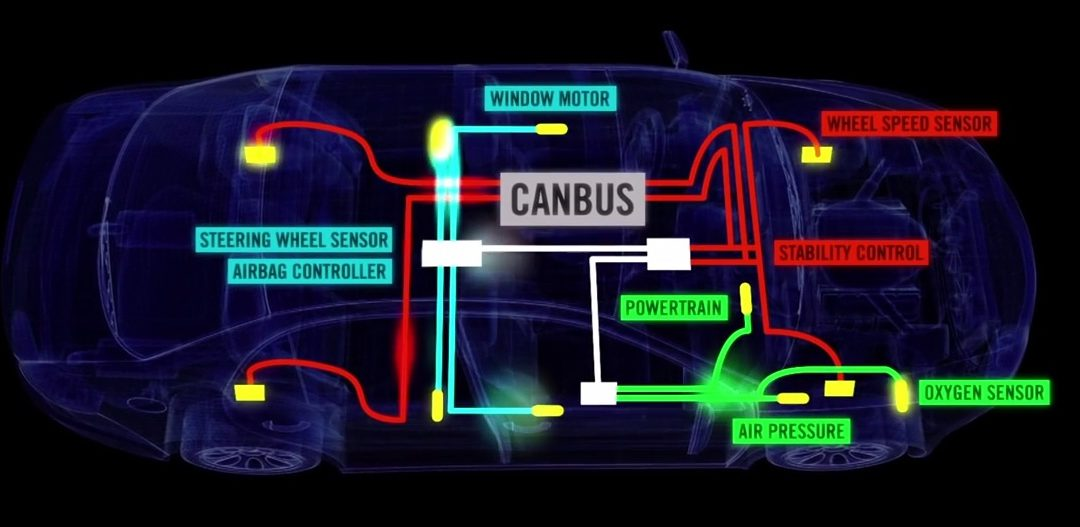
\includegraphics[width=0.5\textwidth]{Ilustraciones/CAN_Car.jpg}
\caption{Imagen ilustrativa de un bus CAN en un vehículo, mostrando la interconexión entre varias ECU a través de un par de cables trenzados. Fuente: \url{https://serviciosdelautomovilarca.es/2021/02/07/sistema-can-bus-en-el-automovil/}.}
\label{fig:CAN_CAR}
\end{figure}


A nivel técnico, el bus CAN es un protocolo de comunicaciones en serie de tipo diferencial, lo que significa que utiliza dos cables (CAN High y CAN Low) para transmitir la información, logrando una excelente inmunidad frente a interferencias electromagnéticas. Funciona bajo un paradigma multimaestro y utiliza un mecanismo de resolución de colisiones no destructivo basado en la prioridad del mensaje (CSMA/CD+AMP). En lugar de enviar información a direcciones específicas, el bus CAN transmite tramas o frames a toda la red. Cada trama contiene un identificador único; cuanto menor es el valor numérico de este identificador, mayor es la prioridad del mensaje en el bus. Esto asegura que la información crítica, como los comandos de frenado, tenga siempre preferencia sobre datos secundarios.\\

\begin{table}[!htbp]
\caption{Estructura de una Trama CAN Estándar 2.0A.}
\label{tab:trama_can}
\centering
\begin{tabular}{|l|c|p{9cm}|}
\hline
\textbf{Campo} & \textbf{Bits} & \textbf{Descripción (Funcionamiento Básico)} \\ \hline
\textbf{SOF} & 1 & \textit{Start of Frame}: Indica el inicio de la transmisión. \\ \hline
\textbf{Identificador (ID)} & 11 & Define la prioridad y el contenido del mensaje. \\ \hline
\textbf{RTR} & 1 & \textit{Remote Transmission Request}: Diferencia entre trama de datos o petición. \\ \hline
\textbf{Control} & 6 & Indica la longitud de los datos que le siguen. \\ \hline
\textbf{Datos} & 0 - 64 & La carga útil (hasta 8 bytes de información, p.ej., valor de RPM). \\ \hline
\textbf{CRC / ACK / EOF} & Varios & Comprobación de errores, confirmación de recepción y fin de trama. \\ \hline
\end{tabular}%
\end{table}

Aunque el bus CAN define cómo viajan los bits por los cables (las capas física y de enlace de datos del modelo OSI), no especifica el "idioma" de los datos en sí. Para que equipos de diagnóstico externos puedan interpretar universalmente la información del vehículo (como las RPM, la temperatura del refrigerante o los códigos de error), la industria adoptó protocolos estandarizados de la capa de aplicación. El más fundamental es el OBD-II (On-Board Diagnostics), obligatorio en Estados Unidos desde 1996 y en Europa (como EOBD) desde principios de los 2000. OBD-II define un conector físico estándar de 16 pines (SAE J1962) y un conjunto de identificadores de parámetros (PID) que cualquier herramienta puede solicitar. Con la llegada de los vehículos modernos, el estándar ISO 15765-4 dictaminó cómo deben encapsularse y enviarse estos mensajes OBD-II a través del bus CAN físico. Además, para diagnósticos más profundos a nivel de fabricante, la industria utiliza actualmente el estándar UDS (Unified Diagnostic Services, ISO 14229), que permite operaciones avanzadas como la lectura de variables propietarias o el flasheo de centralitas.



\section{Introducción a los Protocolos de Comunicación}

El sistema desarrollado en este TFT se apoya en una pila de protocolos estándar 
ampliamente adoptada en el sector de la automoción. Cada capa cumple una función 
específica y bien delimitada, desde la transmisión física de bits hasta la 
interpretación de los datos de diagnosis a nivel de aplicación.


\subsection{CAN Bus \textemdash\ ISO 11898}

El \textit{Controller Area Network} (CAN) es un bus serie multi-maestro desarrollado 
por Robert Bosch GmbH en 1983~\cite{Bosch91-can} y estandarizado bajo la norma 
ISO 11898~\cite{ISO11898-1-15}. Fue diseñado para permitir la comunicación entre 
múltiples unidades de control electrónico (ECUs) a través de un único par de cables 
trenzados, eliminando la necesidad de cableado punto a punto entre 
nodos~\cite{Bosch91-can}. Su mecanismo de arbitraje no destructivo basado en la 
prioridad del identificador de mensaje garantiza que no se produzcan colisiones en el 
bus, mientras que su señalización diferencial lo hace robusto frente al ruido 
electromagnético propio del entorno vehicular~\cite{ISO11898-1-15}. En este proyecto 
se utiliza CAN 2.0A con identificadores de 11 bits a una velocidad de 500 kbps, que 
es la velocidad estándar definida para el acceso OBD-II~\cite{SAE-J1979-12}.


\subsection{ISO-TP \textemdash\ ISO 15765-2}

El \textit{ISO Transport Protocol} (ISO-TP), definido en la norma 
ISO 15765-2~\cite{ISO15765-2-16}, es el protocolo de transporte utilizado sobre CAN 
en el contexto del diagnóstico vehicular. Su función principal es superar la 
limitación fundamental del bus CAN, cuyas tramas admiten un máximo de 8 bytes de 
\textit{payload}~\cite{ISO11898-1-15}: ISO-TP permite segmentar y reensamblar 
mensajes de hasta 4095 bytes mediante cuatro tipos de trama --- \textit{Single Frame} 
(SF), \textit{First Frame} (FF), \textit{Consecutive Frame} (CF) y \textit{Flow 
Control} (FC) ---, que gestionan el flujo de datos entre el escáner y la 
ECU~\cite{ISO15765-2-16}. En este proyecto, ISO-TP actúa como capa de transporte 
imprescindible para transmitir respuestas que exceden los 8 bytes, como el número de 
identificación del vehículo (VIN) o listas de códigos de avería (DTCs), y su 
implementación se apoya en la librería 
\texttt{python-can-isotp}~\cite{Menager23-isotp}.


\subsection{OBD-II \textemdash\ SAE J1979 / ISO 15031-5}

El estándar OBD-II (\textit{On-Board Diagnostics}, segunda generación), definido por 
la SAE J1979~\cite{SAE-J1979-12} y su equivalente europeo ISO 15031-5, establece una 
interfaz de diagnóstico normalizada que cualquier herramienta de escáner puede 
utilizar para interrogar a las ECUs de un vehículo. Sobre CAN, los mensajes OBD-II se 
transportan como \textit{payloads} ISO-TP~\cite{ISO15765-2-16}: el escáner envía una 
petición compuesta por un byte de modo y un byte de PID, y la ECU responde con los 
datos solicitados precedidos por el modo incrementado en 
\texttt{0x40}~\cite{SAE-J1979-12}. El estándar define varios servicios o modos, de 
los cuales este proyecto implementa cuatro: el Modo \texttt{0x01} para la lectura de 
datos en vivo (18 PIDs), el Modo \texttt{0x03} para la lectura de DTCs almacenados, 
el Modo \texttt{0x04} para el borrado de DTCs y el Modo \texttt{0x09} para la 
obtención del VIN del vehículo~\cite{SAE-J1979-12}.


\subsection{UDS NRC \textemdash\ ISO 14229-1}

El estándar UDS (\textit{Unified Diagnostic Services}), definido por la norma 
ISO 14229-1~\cite{ISO14229-1-20}, establece los servicios de diagnóstico de alto 
nivel utilizados en la comunicación entre herramientas de diagnosis y ECUs modernas. 
En el contexto de este proyecto, el elemento relevante de UDS son los 
\textit{Negative Response Codes} (NRC): cuando una ECU no puede atender una 
petición, responde con una trama de respuesta negativa con el formato 
\texttt{[0x7F, modo, código\_NRC]}, donde el código identifica la razón del 
rechazo~\cite{ISO14229-1-20}. Se implementan seis NRCs, entre ellos \texttt{0x11} 
(servicio no soportado), \texttt{0x12} (PID no soportado), \texttt{0x22} 
(condiciones incorrectas, por ejemplo intentar borrar DTCs con el motor en marcha) y 
\texttt{0x33} (acceso denegado por seguridad)~\cite{ISO14229-1-20}, dotando al 
simulador de un comportamiento fiel al de una ECU real.